
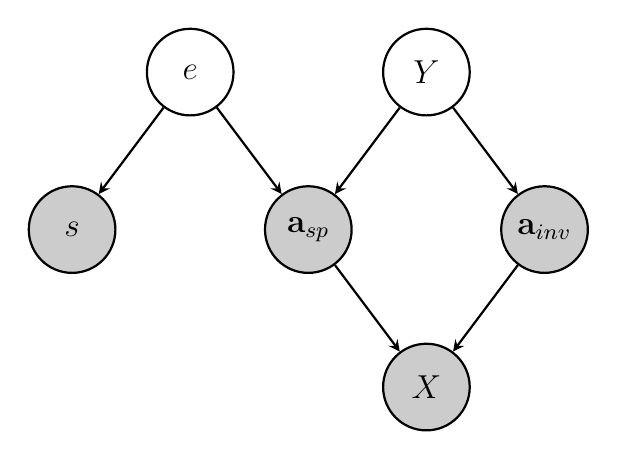
\begin{tikzpicture}[
  every node/.style={draw, circle, minimum size=1.1cm, font=\large},
  shaded/.style={fill=gray!40},
  >=stealth, thick
]

\node[shaded] (s)    at (0, 0)  {$s$};
\node[shaded] (asp)  at (3, 0)  {$\mathbf{a}_{sp}$};
\node[shaded] (ainv) at (6, 0)  {$\mathbf{a}_{inv}$};

\node (e)    at (1.5, 2)  {$e$};
\node (Y)    at (4.5, 2)  {$Y$};

\node[shaded] (X)    at (4.5, -2) {$X$};

% Directed edges
\draw[->] (e)    -> (s);
\draw[->] (e)    -> (asp);
\draw[->] (Y)    -> (asp);
\draw[->] (Y)    -> (ainv);
\draw[->] (asp)  -> (X);
\draw[->] (ainv) -> (X);

\end{tikzpicture}